\subsection{Categorization Graph}
\label{section_cat_graph}

% The objective bounds that the system can be measured against must be set for commit and abort rate percentages and also for the upper and lower bounds for rate of efficiency. A static value could be used for these bounds but then the solution would not be flexible for different environments. Another considered solution could store the category bounds in a relation within the local database but then this approach places the responsibility on the database administrator to ensure the bounds are appropriate for the execution environment. In order to allow the categorization bounds to flex within the execution environment while also allowing the flexibility without the aid of an administrator, we created the categorization graph.

The categorization graph is a graphical representation of the transaction metrics. It is grouped into four sections where each section represents a category that a transaction can be placed. Categorization bounds (see Definition \ref{cat_bounds}) separate the graph into four sections and determine what category the transaction will receive once placed. Transactions are categorized based on the percentages of their previous execution metrics in comparison to the other transactions executing on the same system. This allows the system to flex accordingly with different environments. Depending on the metrics that each transaction possesses, the transactions will be categorized into the previous four categories listed above: $LCLE$, $HCLE$, $HCHE$, and $LCHE$. Transactions categorized as $LCLE$ must have an efficiency rate that is in the 50 percentile or lower where the commit rate is also in the 50 percentile or lower. Transactions categorized as $HCLE$ must have an efficiency rate that is also in the 50 percentile or lower, however, the commit rate must be in the 50 percentile or higher. $LCHE$ transactions must have an efficiency rate that is in the 50 percentile or higher where the commit rate is in the 50 percentile or lower. Transactions categorized as $HCHE$ must have an efficiency rate that is in the 50 percentile or higher where the commit rate is also in the 50 percentile or higher. Figure \ref{graph:cat_graph} and Definition \ref{transaction_categories} show the categorizations described above. The next section outlines the required algorithms for the prediction-based solution.

% \begin{table}[h]
% \captionsetup{justification=centering}
% \centering
% \begin{tabular}{l|c|c|}
% \cline{2-3}
%                                           & \multicolumn{1}{l|}{\textbf{Commit Rate ($C_{r}$)}} & \multicolumn{1}{l|}{\textbf{Efficiency Rate ($E_{r}$)}} \\ \hline
% \multicolumn{1}{|l|}{\textbf{HCHE}}  & $>$ 50\%                          & $>$ 50\%                                \\ \hline
% \multicolumn{1}{|l|}{\textbf{HCLE}}  & $>$ 50\%                       & $\le$ 50\%                               \\ \hline
% \multicolumn{1}{|l|}{\textbf{LCHE}} & $\le$ 50\%                          & $>$ 50\%                                  \\ \hline
% \multicolumn{1}{|l|}{\textbf{LCLE}} & $\le$ 50\%                       & $\le$ 50\%                                 \\ \hline
% %\multicolumn{1}{|l|}{\textbf{No Trnd.}} &    \multicolumn{2}{c|}{See equation below}                                    \\ \hline
% \end{tabular}
% \caption{Transaction Categorization Bounds} % title of the Figure
% \label{tbl:default_tmetrics} % label to refer figure in text
% \end{table}

\begin{figure}[ht]
\captionsetup{justification=centering}
\centering % used for centering Figure
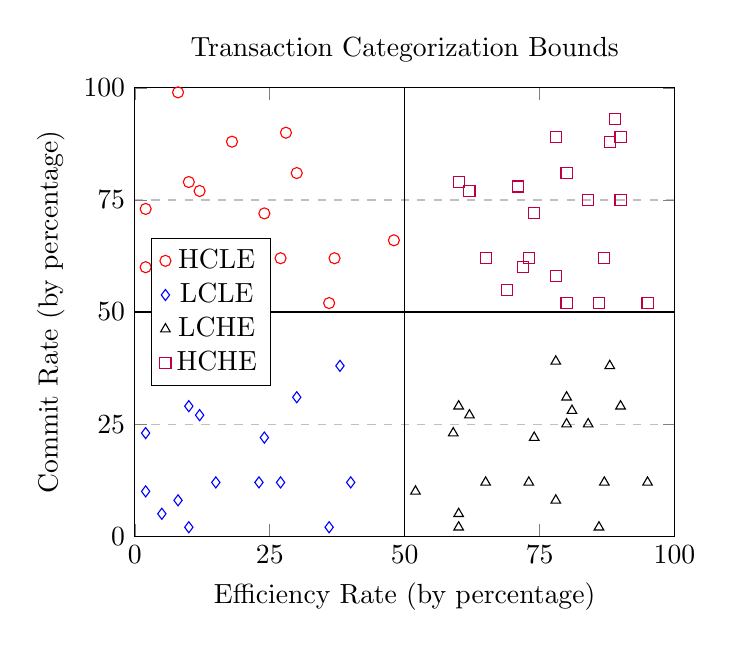
\begin{tikzpicture}
\begin{axis}[
    title={Transaction Categorization Bounds},
    xlabel={Efficiency Rate (by percentage)},
    ylabel={Commit Rate (by percentage)},
    xmin=0, xmax=100,
    ymin=0, ymax=100,
    xtick={0,25,50,75,100},
    ytick={0,25,50,75,100},
    legend style={at={(0.03,0.5)},anchor=west},
    ymajorgrids=true,
    grid style=dashed,
]

% \addplot[
%     color=blue,
%     mark=diamond,
%     ]
%     coordinates {
%     (0,49)(49,49)(49,0)};
% \addplot[
%     color=red,
%     mark=o,
%     ]
%     coordinates {
%     (0,50)(50,50)(50,100)};
% \addplot[
%     color=black,
%     mark=triangle,
%     ]
%     coordinates {
%     (50,0)(50,50)(100,50)};
\draw[-] (0,50) -- (100,50);
\draw[-] (50,0) -- (50,100);
% \addplot[
%     color=purple,
%     mark=square,
%     ]
%     coordinates {
%     (51,100)(51,51)(100,51)};
\addplot[
    only marks,
    color=red,
    mark=o,
    ]
    table {
    10  52
    2   60
    8   58
    5   55
    24  72
    30  81
    15  62
    10  79
    18  88
    28  90
    23  62
    12  77
    37  62
    48  66
    36  52
    8   99
    27  62
    2   73
    };
\addplot[
    only marks,
    color=blue,
    mark=diamond,
    ] 
    table {
    10  2
    2   10
    8   8
    5   5
    24  22
    30  31
    15  12
    10  29
    38  38 
    23  12
    12  27
    40  12
    36  2
    8   49
    27  12
    2   23
    };
\addplot[
    only marks,
    color=black,
    mark=triangle,
    ] 
    table {
    60  2
    52  10
    78  8
    60  5
    74  22
    80  31
    65  12
    60  29
    88  38 
    73  12
    62  27
    95  12
    86  2
    78  39
    87  12
    59  23
    80  25
    81  28
    84  25
    90  29
    };
\addplot[
    only marks,
    color=purple,
    mark=square,
    ] 
    table {
    80  52
    72  60
    78  58
    69  55
    74  72
    80  81
    65  62
    60  79
    88  88 
    73  62
    62  77
    95  52
    86  52
    78  89
    87  62
    89  93
    90  75
    71  78
    84  75
    90  89
    };

\legend{HCLE, LCLE, LCHE, HCHE}
 
\end{axis}
\end{tikzpicture}
\caption{Categorization Graph} % title of the Figure
\label{graph:cat_graph} % label to refer figure in text
\end{figure}